\documentclass[landscape,blockverticalspace=0mm,20pt]{awe-tikzposter}

\usetheme{Simple}
\usecolorstyle[colorPalette=York]{Denmark}

\usepackage{graphicx}
\graphicspath{{../figures/}{./}}

\setlength{\columnsep}{10ex}

\usepackage{multicol}

\RequirePackage{unicode-math}
\setmathfont[Script=Math]{Tex Gyre Pagella Math}
\setmathfont[range=\mathup,Numbers=Lining]{Linux Biolinum}


% \logo{penn-logo}

% \qrcode{qr}

\title{Algorithmic generation of random languages argues for syntax as a source of phylogenetic information}
\author{A.~Ceolin​, ​A.~Ecay​, ​C.~Guardiano​, ​M.~A.~Irimia​, G.~Longobardi​, ​D.~Michelioudakis​ and ​N.~Radkevich}
\institute{University of York and University of Modena and Reggio Emilia (CG)}
\date{May 29, 2015}

\begin{document}

\poster{\maketitle[width=0.8\paperwidth]}

\begin{columns}
    \column{0.25}

    \block{Introduction}{%
        \begin{itemize}
          \item The \textbf{Classical Comparative Method} (CCM): build
            language phylogenies based on sound laws.  Very successful
            over \textasciitilde{}10k years (IE, Austroneisan, Bantu,
            ...), but does not extend further back in time.
          \item Recent extensions of the CCM use \textbf{computational
                methods} to augment its conclusions (Dyen et al 1992,
            Ringe et al 2002, Gray and Atkinson 2003, Bouckaert et al
            2012).  These too ran into the time limit imposed by
            \textbf{lexical decay}: the tendency of words to change
            meaning and die out over time
          \item The \textbf{Parametric Comparison Method} (PCM;
            Guardiano and Longobardi 2005) proposes the use of syntax
            for historical comparison and reconstruction.
        \end{itemize}
        \innerblock{Why Syntax?}{%
            \begin{itemize}
              \item It is universal
              \item It is comparable across language families (no worry
                about “cognates” in syntax)
              \item It may be conservative (especially in the nominal
                domain)
              \item It can be parameterized through syntactic theories
            \end{itemize}
        }
        \begin{itemize}
          \item Other attempts to use syntax for comparison have
            focused on \textbf{surface properties} (Dunn et al 2011).
            However, we know that these surface properties may have
            different syntactic – and thus historical – explanations.
          \item The PCM distills surface properties into underlying
            abstract parameters, taken from the syntax of the DP.
        \end{itemize}
    }

    \block{Parametric implications}{%
        \begin{itemize}
          \item Parameters are not all independent.  Rather, the values
            of certain parameters can depend on others.
        \end{itemize}
        \innerblock{Two types of implications}{%
            \begin{itemize}
              \item \textbf{Empirical implications}: for example,
                languages which do not grammaticalize person do not
                grammaticalize gender (cf.~Greenberg 1963, Universal 36)
              \item \textbf{Logical implications}: for example,
                in languages which do not have a definite article, it
                cannot be determined whether they have a suffixal
                definite article
            \end{itemize}
        }
        \begin{itemize}
          \item Our parameterization of languages is thus
            \textbf{ternary}; possible values are +, $-$, or 0
            (implied).
          \item Implications sharply reduce the number of possible
            languages: from $2^{62} = 4.6 \times 10^{18}$ to $1.4 \times
            10^{10}$ (Bortolussi et al)
          \item This solves the problem of exponential complexity for
            learners raised by Clark \& Roberts (2003), Lightfoot (2006)
            and Wexler (2011), among others
          \item This system of implications is similar to the proposals
            of Biberauer \& Roberts (2012) about the granularity of
            parameters and learners’ decisions when setting them
        \end{itemize}
    }

    \column{0.25}

    \block{Distance- vs.~character-based methods}{%
        \begin{itemize}
          \item There are two major families of computational methods
            for constructing phylogenetic trees: \textbf{distance-based}
            and \textbf{character-based}
          \item Character-based methods depend heavily on \textbf{shared
            innovations}
          \item Character-based methods are not apt for our data for
            three reasons:
            \begin{enumerate}
              \item \textbf{No model of syntactic evolution}: unlike
                with phonological comparisons where there are strong
                models (mergers are irreversible), there is no model of
                the evolution of syntax which allows us to identify
                shared innovations in principle
              \item \textbf{Effects of non-phylogenetic signals}:
                parallel development, borrowing, and back-mutation are
                concerns for character-based methods.  The low number of
                possible values for syntactic parameters is a challenge:
                every change goes from + to $-$ or vice versa.  Thus it
                is difficult to identify individual changes (unlike with
                DNA, where there are three values to change to)
              \item \textbf{Effects of implications}: Certain
                macroparameters can close off large swaths of others.
                If one of these parameters changes, then it could hide
                shared innovations
            \end{enumerate}

          \item By condensing information to a single distance value,
            distance-based methods overcome these problems
        \end{itemize}
    }

    \block{Sampling}{%
        \begin{itemize}
          \item Bortolussi et al (2011) used an algorithm to randomly
            sample from a uniform distribution of languages compatible
            with parametric implications
          \item This leads to an unbalanced distribution over parameter
            values
          \item We have updated this algorithm to sample parameters in a
            balanced way
        \end{itemize}
    }

    \block{Dataset}{%
        \begin{itemize}
          \item The data for this presentation come from a database of
            75 parameters and 40 languages
          \item 24 IE, 2 Semitic, 3 Finno-Ugric, 2 Basque varieties, 2
            Sino-Tibetan, 2 Altaic, Inuktitut, Japanese, Kuikuro
            (Karib), Kadiweu (Mataco-Guaicuru), and Wolof (Niger-Congo)
        \end{itemize}
    }

    \block{Conclusions}{%
        \begin{itemize}
          \item Syntax is a useful tool for phylogenetics, even at
            long time depths
          \item Parametric theories are especially amenable to
            formalization through mathematical models
          \item In Eurasian languages, a (faint) historical signal is
            present beyond the family level
          \item We cannot yet say whether this is due to descent,
            borrowing, or parallel development
        \end{itemize}
    }

    \column{0.25}

    \block{Language distribution}{%
        \begin{itemize}
          \item Figure~\ref{fig:dist} shows the distribution of observed
            language distances, as well as simulated distances from a
            population of 5,000 languages (12.5M distances)
        \end{itemize}

        \begin{awetikzfigure}{fig:dist}{A plot of the distributions of
                simulated and observed language distances}
            \includegraphics[width=\colwidth]{distributions-poster}
        \end{awetikzfigure}

        \begin{itemize}
          \item The distances are noticeably smaller than the random
            distribution.  This effect remains if we calculate the
            distribution only of pairs which do not belong to a recognized
            language family
          \item This demonstrates that the lingusitic distances
            \textbf{carry historical signal}
        \end{itemize}
    }

    \block{Long-range signal}{%
        \begin{itemize}
          \item We can set a threshold for distances that are “close”
          \item 0.21, or 1/1,000 random languages – probably
            chance-proof
          \item 39\% of our language pairs fall in this region
          \item Including many pairs between IE and its neighbors: see Figure~\ref{fig:bars}
        \end{itemize}
        \begin{awetikzfigure}{fig:bars}{A plot of cross-family distances
            below a threshold value.}
            \includegraphics[width=\colwidth]{close-pair-bars-poster}
        \end{awetikzfigure}
        \begin{itemize}
          \item A $\chi^2$ test confirms that there is a meaningful
            concentration of low distances in Eurasian language pairs ($p
            = 6.7 \times 10^{-12}$)
        \end{itemize}
    }

    \column{0.25}

    \block{A tree}{
        \begin{itemize}
          \item We can use a phylogenetic algorithm to produce a tree
            from our data, seen in Figure~\ref{fig:tree}
        \end{itemize}
        \begin{awetikzfigure}{fig:tree}{A tree produced by KITSCH from
                our data}
            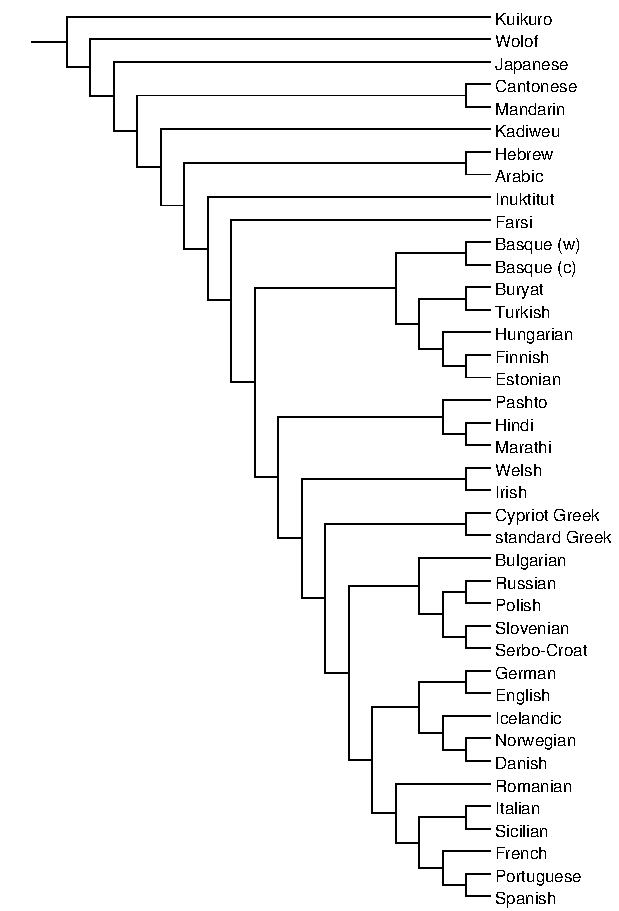
\includegraphics[width=\colwidth]{tree-final-cropped}
        \end{awetikzfigure}
        \begin{itemize}
          \item The tree produces a substantially correct tree for IE,
            with correct internal articulation
          \item It additionally produces a Finno-Ugric/Altaic clade
          \item Problems:
            \begin{itemize}
              \item Basque is classified with Finno-Ugric and Altaic
                \begin{itemize}
                  \item Highly dependent on specific languages
                    (Estonian) and parameters (head-marking genitives)
                \end{itemize}
              \item Farsi is classified outside of IE
                \begin{itemize}
                  \item Evidence of an areal effect on Farsi in
                    linguistic as well as genetic terms
                \end{itemize}
            \end{itemize}
        \end{itemize}
    }

\end{columns}

\end{document}
